\documentclass[12pt]{article}
\usepackage[spanish]{babel}
\usepackage{makeidx}
\usepackage[margin=1in]{geometry}  % set the margins to 1in on all sides
\usepackage{graphicx}              % to include figures
\usepackage{amsmath}               % great math stuff
\usepackage{amsfonts}              % for blackboard bold, etc
\usepackage{amsthm}                % better theorem environments
\usepackage{makeidx}               % index
\usepackage[utf8]{inputenc}        % now we have tildes!
\usepackage{wrapfig}               % images
\usepackage{listings}              % Unordered lists
\usepackage{hyperref}              % hyperlinks
\usepackage{xcolor}                % to colorize font
\usepackage{blindtext}             % to colorize font

% Color definitions
\definecolor{landanimal}{rgb}{.545,.1,.1}
\colorlet{ocean}{blue!60!black}
\newcommand{\earth}[1]{\textcolor{landanimal}{#1}}
\newcommand{\water}[1]{\textcolor{ocean}{#1}}

\makeindex

\begin{document}

\begin{titlepage}

\newcommand{\HRule}{\rule{\linewidth}{0.5mm}} % Defines a new command for the horizontal lines, change thickness here

\center % Center everything on the page

%----------------------------------------------------------------------------------------
%	HEADING SECTIONS
%----------------------------------------------------------------------------------------

\textsc{\LARGE Universidad Carlos III de Madrid}\\[1.2cm] % Name of your university/college


\includegraphics[width=9cm]{Logo}\\[1.2cm] % Include a department/university logo - this will require the graphicx package

\textsc{\Large Aprendizaje Automático}\\[0.5cm] % Major heading such as course name
\textsc{\large Grado en Ingeniería Informática}\\[0.6cm] % Minor heading such as course title
\textsc{\large Grupo 83}\\[0.5cm]

%----------------------------------------------------------------------------------------
%	TITLE SECTION
%----------------------------------------------------------------------------------------

\HRule \\[0.7cm]
{ \huge \bfseries Práctica 1: Clasificación y Predicción}\\[0.4cm] % Title of your document
\HRule \\[1.3cm]

%----------------------------------------------------------------------------------------
%	AUTHOR SECTION
%----------------------------------------------------------------------------------------


% If you don't want a supervisor, uncomment the two lines below and remove the section above
\emph{Autores:}\\
Daniel \textsc{Medina García}\\ % Your name
Alejandro \textsc{Rodríguez Salamanca}\\[1.5cm] % Your name

%----------------------------------------------------------------------------------------
%	DATE SECTION
%----------------------------------------------------------------------------------------

{\large \today}\\ % Date, change the \today to a set date if you want to be precise

%----------------------------------------------------------------------------------------
%	LOGO SECTION
%----------------------------------------------------------------------------------------



%----------------------------------------------------------------------------------------

\vfill % Fill the rest of the page with whitespace

\end{titlepage}

\tableofcontents

\newpage
\thispagestyle{empty}
\clearpage
\vspace*{\fill}
\begin{center}
    \begin{minipage}{\textwidth}
        \begin{center}
            \section*{Motivación}
            En esta primera práctica, nuestro equipo de trabajo emplea los conocimientos adquiridos en los anteriores \emph{Tutoriales} para implementar un agente automático que utiliza técnicas de aprendizaje automático para su funcionamiento. Vistas las restricciones que causaba no poder utilizar estas técnicas en el \emph{Tutorial 1}, es ahora el momento de probar si realmente suponen una ventaja o no a la hora de implementar un agente automático para el famoso \emph{PacMan}. ¿Merece la pena el uso de estas técnicas para este juego? ¿Qué datos son de utilidad y cuáles no para implementar un agente que trabaje con aprendizaje automático? ¿Cómo nos ayuda tratar de predecir las futuras jugadas a la hora de elegir nuestro movimiento? Estas y otras cuestiones serán tratadas en la memoria que está a punto de leer. En ella se explica en detalle el proceso seguido para conseguirlo, en el que se generarán modelos de clasificación para la elección del movimiento y modelos de regresión para la elaboración de predictores.
        \end{center}
    \end{minipage}
\end{center}
\vfill

\newpage
\section{Fase 1: Instancias de Entrenamiento y Test}

\subsection{Función para la extracción de características}

Lo primero que necesita el modelo de clasificación que decidirá la siguiente acción a tomar por el agente automático son \textbf{datos}: un historial de datos lo suficientemente significativo para poder responder ante cualquier situación posible dentro del juego y así tomar la dirección acertada.

Para extraer los datos del juego, se partió de la función utilizada en el tutorial anterior. Ésta recopilaba tan sólo datos disponibles en el momento actual acerca de la situación de los agentes, tanto \emph{PacMan} como los codiciados fantasmas, y no seguía el formato de la herramienta que posteriormente emplearíamos para la minería de los datos, \emph{Weka}. Esa base fue ampliada mediante la experimentación, añadiendo, modificando y eliminando atributos según mejoraba o empeoraba el éxito de clasificación del árbol resultante con distintos algoritmos, como será explicado en la \emph{Fase 2}, y se adaptó para generar el archivo con los contenidos necesarios (cabeceras y formato) para ser reconocido por \emph{Weka}.

\subsection{Función para la extracción de características de situaciones futuras}

Una de las principales diferencias de la base respecto a la función de recopilación de datos que utilizamos en este tutorial es la recopilación de datos futuros en las instancias del fichero \texttt{.arff} que genera el recopilador. Para implementar esta funcionalidad, se ha utilizado un método de escritura retardada. Así, no se escribe una nueva línea en el fichero hasta que no se conocen todos los datos que se han de escribir, almacenando mientras tanto los datos intermedios. Esto se hizo creando listas globales, que almacenan las líneas incompletas (a falta de datos futuros) en \texttt{future\_lines} y las puntuaciones (para completar las líneas anteriores cuando llegue su turno) en \texttt{future\_score}. Cuando la primera línea esté completa (en este caso, en el sexto turno), se imprimirán en el archivo los datos que ya se tenían junto a los recién llegados, creando así una línea completa.

\subsection{Extracción de datos}

Con el fin de preparar los datos sobre los que construir un modelo de clasificación, en este punto se recopilaron los datos de juego utilizando la función mencionada anteriormente. Para ello, se elaboró un \emph{script} que hacía jugar al agente automático un determinado número de partidas de forma autónoma y ---ya que, lamentablente, no tenemos becarios--- los miembros del equipo jugaron asimismo el mismo número de partidas. De esta manera recopilamos tanto jugadas del agente automático como del controlado por un humano, y además generamos archivos con datos adicionales futuramente empleados como conjuntos de test.

Todos estos ficheros, así como más que fueron generados en los procesos de experimentación de las siguientes fases, pueden encontrarse en el material proporcionado junto a este documento.

\newpage
\section{Fase 2: Clasificación}

\subsection{Transformación de datos}

Es este el factor donde el razonamiento sobre los datos puede dar lugar a más variantes. Ya que anteriormente no se han comentado, mencionamos aquí la base de atributos de los que partimos:
\begin{itemize}
    \item \texttt{score} : puntuación actual de \emph{PacMan}.
    \item \texttt{ghost<N>-living} : True si el fantasma $N$ sigue vivo, False si ya ha sido comido.
    \item \texttt{distance-ghost<N>} : Distancia ruidosa de \emph{PacMan} al fantasma $N$.
    \item \texttt{posX} y \texttt{posY} : Coordenadas de \emph{PacMan} sobre el tablero.
    \item \texttt{direction} : Hacia dónde mira \emph{PacMan} (último movimiento realizado).
    \item \texttt{wall-<direction>} : `True' si hay un muro en \textless direction\textgreater, False si vía libre.
    \item \texttt{move} : Movimiento tomado en el turno, es la \textbf{clase}.
\end{itemize}

La experimentación ha sido la protagonista en esta fase. Lamentablemente, su protagonismo se ha debido a la búsqueda de nuevas alternativas ante las numerosas pruebas descartadas por ausencia de resultados positivos, como son explicadas a continuación.

\vspace{0.2cm}

Tratamos de agregar los datos que teníamos de forma que resultasen en algún campo útil para el modelo, y para ello probamos a convvertir los atributos \texttt{ghost<N>-living} en uno sólo que fuese la suma de los fantasmas vivos (aplicando primero el filtro \emph{NominalToBinary} sobre los cuatro atributos, y luego el filtro \emph{AddExpression} sumándolos todos). No obstante, el resultado fue un un decremento de éxito de clasificación de entre el 2.3\% y el 3\%, dependiendo del método utilizado para la evaluación.

\vspace{0.2cm}

Consideramos también la generalización de nuestro agente a un número $N$ de fantasmas. El agente base es válido sólo para partidas con 4 fantasmas, si bien el juego real puede constar de un número distinto de ellos. Para solucionar el problema de jugar con más de cuatro fantasmas, se podrían considerar siempre los 4 fantasmas más cercanos (i.e. los ``mejores''). Pero, ¿y si fueran menos? Podríamos reducir ese 4 hasta 1, de forma que sólo se tuviese en cuenta el fantasma más cercano y el agente siempre fuese a por él obviando a los demás. Si vemos hacia dónde nos está llevando esta línea, observamos que estamos sobredirigiendo el aprendizaje y acabamos imitando al agente del \emph{Tutorial 1}. Por ello, abandonamos estas hipótesis por, en nuestra opinión, alejarse de los objetivos de la práctica.

\newpage
\subsection{Experimentación y comparaciones}

En esta fase el equipo dedicó su esfuerzo a realizar tantas pruebas como fuesen posibles, probando diferentes combinaciones de algoritmos, filtros y atributos para generar el modelo basándonos en conocimiento y razonamientos \emph{a priori}.

\vspace{0.2cm}

Para crear un modelo exitoso, hay que tener en cuenta varios factores, a continuación analizaremos cada uno de ellos:

\subsubsection{Elección de los datos de entrada para la creación del modelo}

Para la elección de la entrada para el algoritmo, partimos de dos bases: los datos de ejecución del agente automático (que, para jugar, se informa tan sólo de los sensores que le indican las distancias a cada uno de los fantasmas) y los de las partidas que jugamos los miembros del equipo, viendo los fantasmas. No es difícil llegar a la conclusión de que el agente humano gana las partidas mucho más rápido que el agente implementado en el \emph{Tutorial 1}, pero eso no tiene por qué indicar que necesariamente los datos del agente de teclado generasen un modelo con un mayor éxito de clasificación. Sin embargo, con posteriores pruebas encontramos un aplastante 10-15\% de diferencia en éxito de clasificación a favor del agente de teclado entre los modelos generados para ambos archivos con \emph{J48} y \emph{BFTree}, dos de los algoritmos que conocíamos de tutoriales anteriores y sabíamos generaban árboles bastante buenos, evaluados con cross-validation. La siguiente tabla ilustra los resultados obtenidos:

\begin{center} 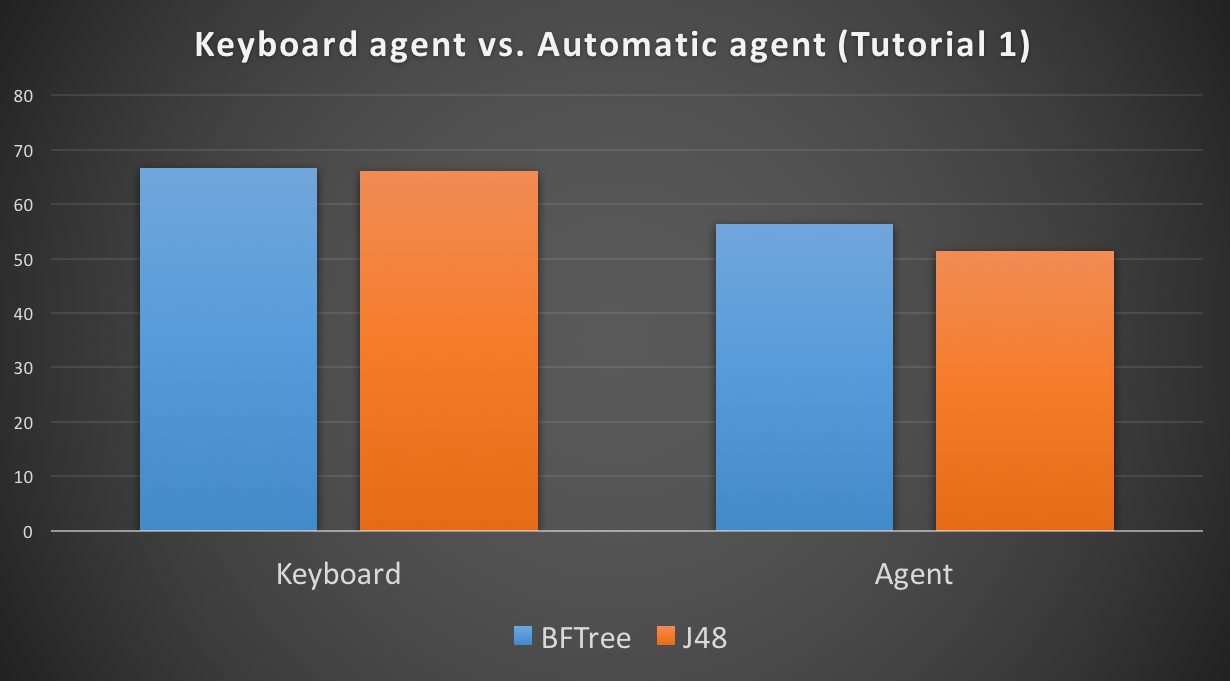
\includegraphics[width=14cm]{kb_vs_aa} \end{center}

Viendo estos datos, nos decantamos por \texttt{training\_keyboard\_edited.arff}, que es el fichero que contiene los datos legales (sin los datos de puntuaciones futuras), para generar el modelo en \emph{Weka}.

\newpage
\subsubsection{Elección del algoritmo generador de nuestro modelo}

Una vez escogido el archivo que se usará para generar el modelo, comenzamos la comparación entre algoritmos para realizar dicha tarea. Para ello, comparamos varios algoritmos de creación de árboles de decisión evaluándolos tanto con validación cruzada como con dos sets de instancias generadas en partidas jugadas, uno en los mismos mapas que en el entrenamiento y otro en mapas distintos. El éxito de clasificación de cada uno de los algoritmos utilizados se muestra en la siguiente tabla:

\vspace{0.2cm}

\noindent 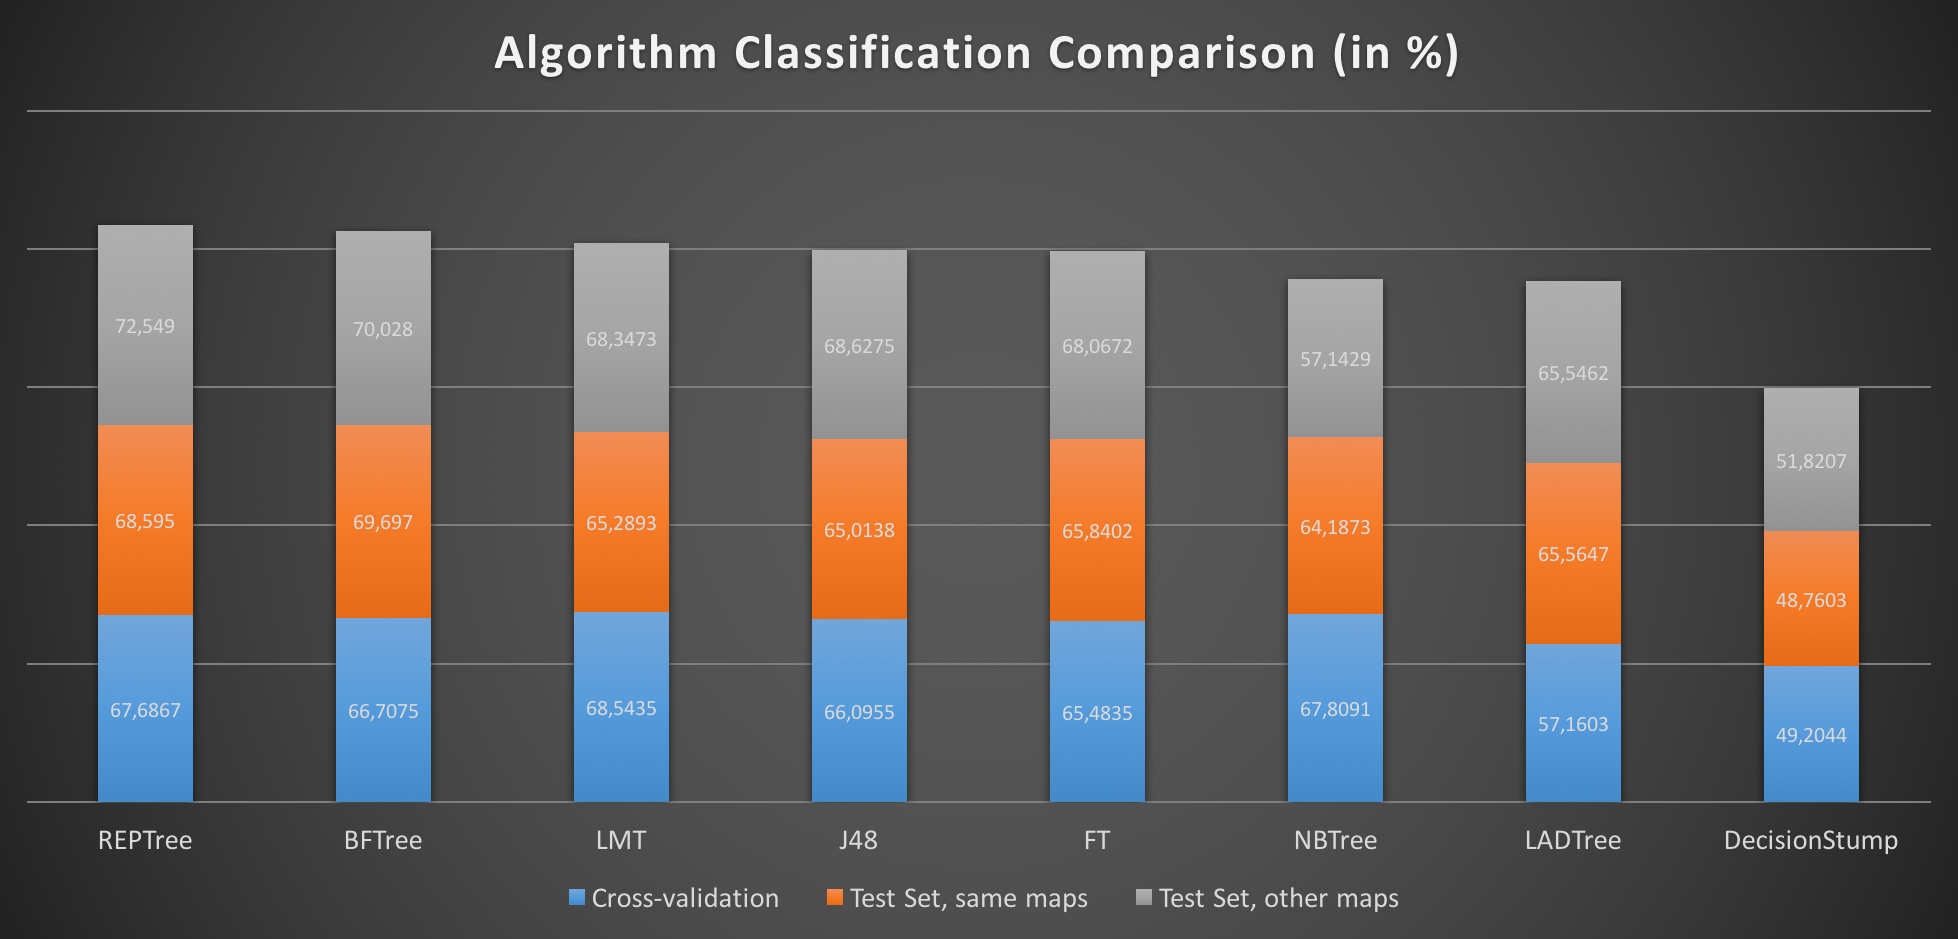
\includegraphics[width=\textwidth]{algorithm_comparison}

\vspace{0.2cm}

Nos sorprendieron los resultados de \emph{REPTree}, un algoritmo que no habíamos utilizado con anterioridad y, sin embargo, obtuvo los mejores resultados. Si bien este algoritmo suele utilizarse para clasificaciones multi-clase, esto no le impide funcionar para una sola clase también, y queda demostrado que con efectividad. Esta información se tendrá muy en cuenta a la hora de elegir el algoritmo generador del modelo en el cual se basará nuestro nuevo agente automático para tomar las decisiones pertinentes, y nos sirve para descartar algunos algoritmos, agilizando los cómputos posteriores.

\subsubsection{Aplicación de filtros para mejorar el comportamiento de los algoritmos}

Intentamos extraer el máximo de información de los datos que ya teníamos, sesgándolos mediante la aplicación de filtros que pudiesen acarrear un mejor funcionamiento de los algoritmos de prueba.

Como el movimiento \texttt{STOP} no aporta valor al juego (no conseguirá acercarse a ningún fantasma), editamos nuestro fichero de datos eliminando las instancias que hubiesen realizado ese movimiento (i.e. aquellas transcurridas entre que empieza el juego y el jugador de teclado pulsa la primera tecla, ya que es el único momento en el que se produce este hecho) por considerarlas ruidosas. Una vez completada esta primera ``purga'', procedimos a balancear las instancias de cada clase para tener un número similar de instancias que realizasen cada movimiento. Estos fueron los resultados obtenidos en cuanto a éxito de clasificación según los modelos generados:

\newpage
\noindent 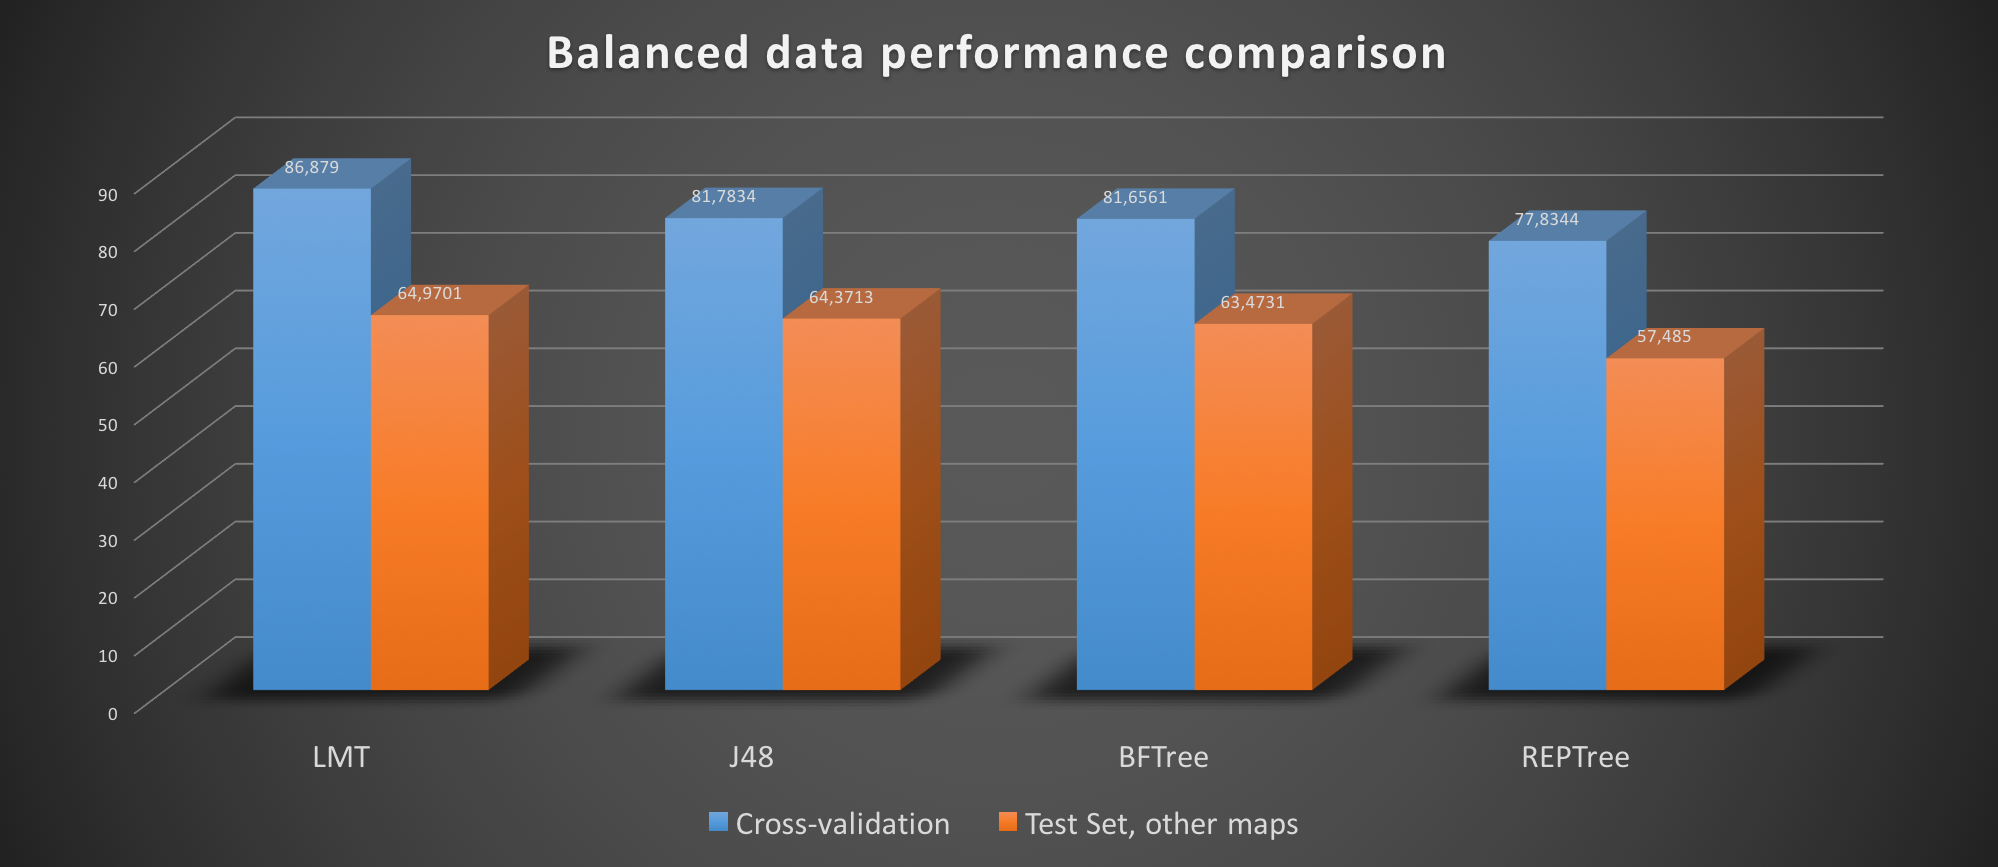
\includegraphics[width=\textwidth]{balanced_performance}

\vspace{0.3cm}

Si bien observamos una clara mejora (de entre el 10 y el 20\%) cuando evaluamos los modelos con validación cruzada, los resultados son desfavorables al evaluar los modelos con una pila de instancias adicional tomadas en otros mapas, decrementando entre un 1 y un 11\% el éxito en clasificación cuando lo comparamos con los datos en bruto.

\subsection{Implementación}

Para la implementación del agente automático teníamos dos opciones: escoger uno de los modelos que hemos obtenido previamente con \emph{Weka} e implementarlo manualmente, o usar un wrapper de \emph{Weka} para \texttt{Python} que, dado un modelo en un fichero \texttt{.model} (o un fichero \texttt{.arff} a partir del cual generarlo), nos devuelva la clase a la que pertenece una instancia dada.

En nuestro caso, decidimos escoger la segunda opción por varios motivos. Primero, porque queríamos experimentar cómo funcionan \texttt{Python} y \emph{Weka} juntos, ya que \emph{Weka} está desarrollada en \texttt{Java}; y segundo porque nos parecía un enfoque mucho más interesante y eficiente, pues de esta forma es más sencillo probar diferentes agentes sin necesidad de reescribir todo el código del agente en cuestión.

Para poder usar \emph{Weka} en \texttt{Python} debemos usar un Wrapper\footnote{https://pythonhosted.org/python-weka-wrapper/}. Una vez que se han seguido los pasos que dan para su instalación ---ya que es necesario instalar una serie de librerías para que todo funcione correctamente--- y configurado el entorno, debemos abrir nuestro fichero de datos e indicarle a \emph{Weka} cuál de los atributos de este fichero es la clase. Por convención, es común que la clase sea el último atributo de una instancia y, como este es nuestro caso, simplemente llamamos al método \texttt{class\_is\_last()} para indicar que efectivamente nuestra clase se encuentra en la última posición de nuestros datos.

\newpage

Para realizar la clasificación, \emph{Weka} proporciona \texttt{Clasifier}, donde se le puede indicar qué algoritmo queremos usar. Por ejemplo, si queremos usar \emph{J48}, nuestra creación de la instancia del clasificador deberá ser \texttt{Classifier(classname="weka.classifiers.trees.J48", options=["-C", "0.3"])}. El modelo generado por este clasificador se escribe en un fichero con extensión \texttt{.model}, y podrá ser usado posteriormente para clasificar nuevas instancias. Fue en la parte de uso de dicho modelo es en la que hemos encontrado más dificultades, puesto que \emph{Weka} no está pensado para clasificar instancias en tiempo de ejecución, sino para tratar ficheros de datos \emph{estáticos}, que no van cambiando a medida que se ejecuta un programa.

\vspace{0.5cm}

Nuestra primera idea tras investigar en los ejemplos publicados del uso del wrapper, mirar en la documentación y preguntar al profesor fue emplear los métodos \texttt{create\_numeric} y \texttt{create\_nominal} de la clase \texttt{Attribute} para crear e indicar nombre y tipo de los datos de nuestra instancia. Después, se inicializa la instancia con \texttt{Instance.create\_instance} para posteriormente pasársela al clasificador. A este método se le pasa una lista en la que cada posición se corresponde con el valor de un atributo. En principio, tenía mucho sentido que esta implementación funcionase, pero \emph{Weka} por debajo convierte los datos de tipo nominal a \texttt{float} y, en este caso, no era capaz de realizar una conversión o un mapeo de \texttt{string} a \texttt{float}. En este punto, lo siguiente que probamos fue realizar nosotros mismos este \emph{mapeo}, usando un diccionario, pero nuevamente surgían errores que no llegábamos a comprender del todo, así que finalmente cambiamos totalmente el enfoque para solucionar el problema.

\vspace{0.5cm}

En el segundo intento de implementar el clasificador de nuevas instancias, la parte de generar el modelo es exactamente igual que la descrita antes. Sin embargo, probamos una nueva forma de pasar nuestros datos en \emph{raw} a instancias que \emph{Weka} es capaz de comprender. Para ello, escribimos en un archivo las cabeceras de \emph{Weka} que contienen los datos y su tipo, y después escribimos una línea con los datos de nuestra instancia, con la particularidad de que el valor de la clase es una interrogación (?). Esto le indica a \emph{Weka} que no sabemos el valor de la clase. A continuación, cargamos el archivo que acabamos de escribir y obtenemos nuestra instancia gracias al método \texttt{classify\_instance()} de la clase \texttt{Classifier}. Este método devuelve un \texttt{float} ---se ve que esta vez \emph{Weka} sí que es capaz de realizar la conversión de nominal a float...--- que se corresponde con el índice del valor de la clase en su declaración en la cabecera del archivo. Finalmente, devolvemos la dirección correspondiente si está dentro del conjunto de direcciones permitidas, o una de las direcciones adyacentes a esta en su defecto (si el resultado es \emph{North}, pero no está permitida, devolveremos \emph{East} o \emph{West}).

\newpage
\section{Fase 3: Predicción}

Para iniciar esta nueva fase, partimos de los datos que ya seleccionamos en la \emph{Fase 2}, i.e. los datos del agente de teclado, pero esta vez sí podremos utilizar los atributos \texttt{score2} y \texttt{score5} para los predictores de la puntuación dentro de dos y cinco jugadas, respectivamente.

\subsection{Transformación de datos}

Antes de considerar el resto de atributos, queremos razonar sobre la exclusión o inclusión de la clase en el modelo de predicción para puntuaciones futuras. Si bien la inclusión de \texttt{move} seguramente resulte en una mejoría en la regresión, esta será despreciable teniendo en cuenta que sí se está analizando el movimiento anterior (a través del atributo \texttt{direction}) y, por el contrario, implicaría la inutilidad del predictor a la hora de generar el valor para el atributo de la puntuación futura ya que sólo podría generar la predicción después de clasificar la instancia, que es para lo que está pensado. Siguiendo este razonamiento, hemos optado por \textbf{excluir la clase en el predictor}, y así poder utilizarlo en nuestro agente.

Además de este cambio sobre los datos para los dos predictores que vamos a implementar (puntuación para 2 y 5 turnos vista, respectivamente), para cada uno de ellos debemos eliminar también el campo opuesto. Así, para el predictor de $N=2$ eliminaremos \texttt{score5} y viceversa.

\subsection{Experimentación y comparaciones}

Siguiendo la motivación de la \emph{Fase 2}, planteamos distintas alternativas para mejorar el rendimiento de nuestro predictor a la hora de clasificar. Pueden observarse en la siguiente gráfica los resultados de los distintos modelos de regresión generados con \emph{REPTree} para predecir a 2 y 5 turnos vista, donde se demuestra nuestra hipótesis respecto a la exclusión de \texttt{move}: el empeoramiento en términos de rendimiento del algoritmo es despreciable.

\vspace{0.3cm}

\noindent 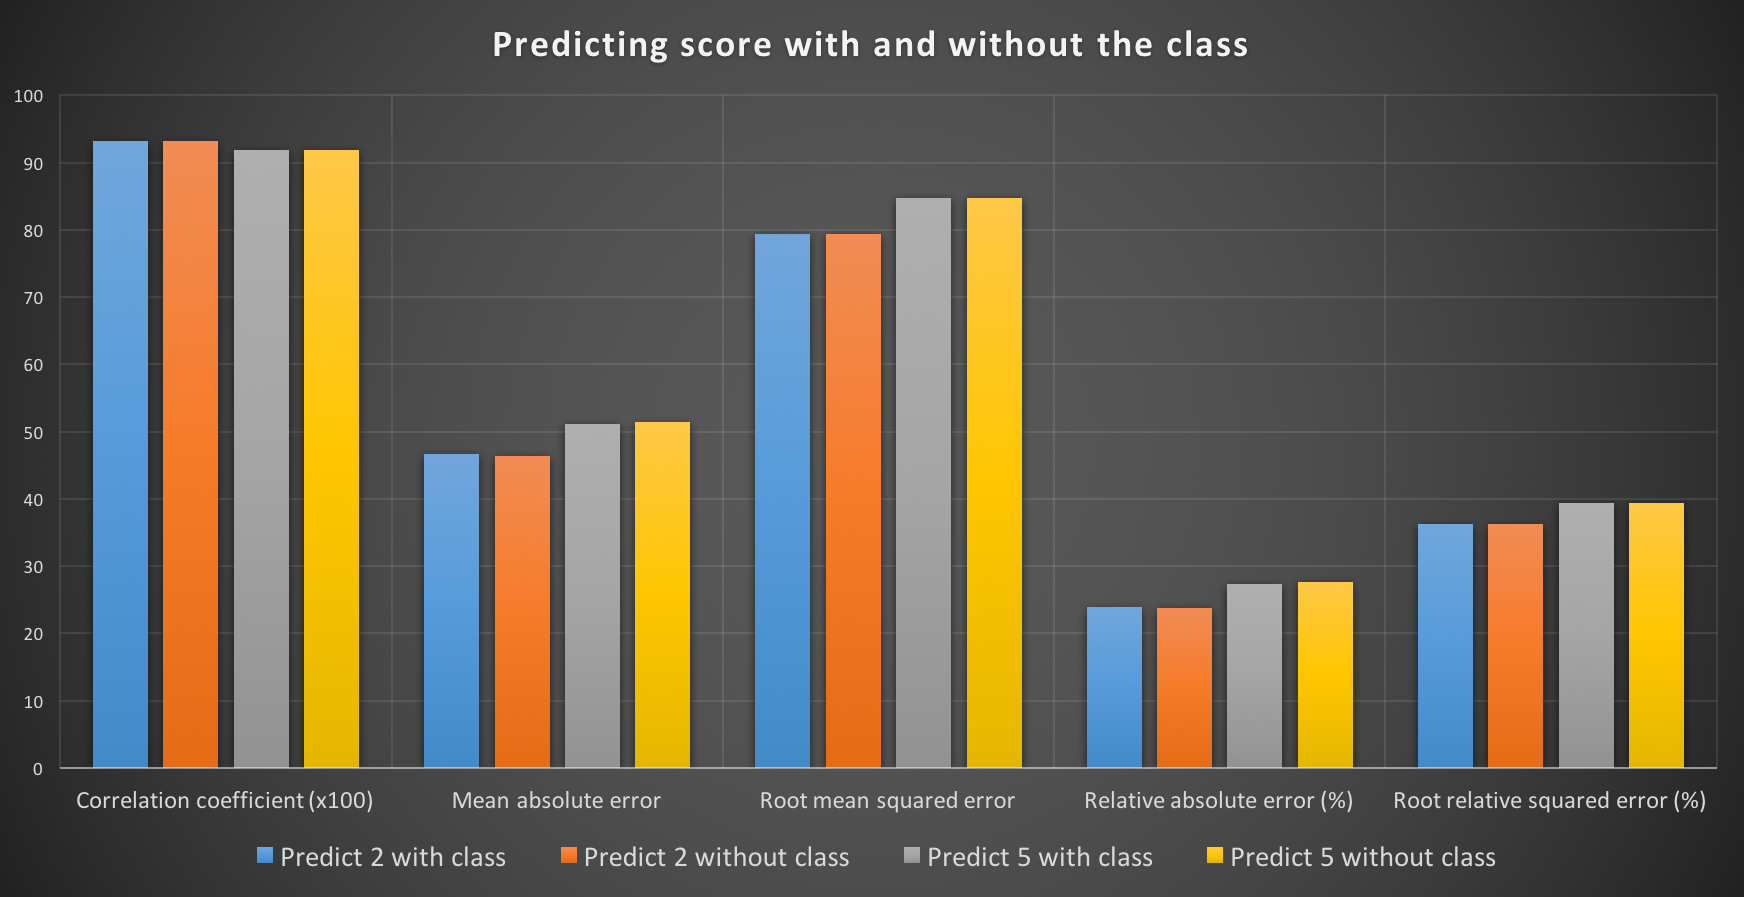
\includegraphics[width=\textwidth]{class_or_no}

\newpage

No contentos con este hallazgo, procedemos ahora a comparar también el algoritmo que utilizamos en la \emph{Fase 2} con otro nuevo, \emph{M5}. Ya que \emph{REPTree} es el único algoritmo capaz de dar una regresión como resultado de los utilizados en la fase anterior, nos vemos obligados a buscar nuevos algoritmos que comparar. La siguiente gráfica compara sendos generadores de modelos:

\vspace{0.3cm}

\noindent 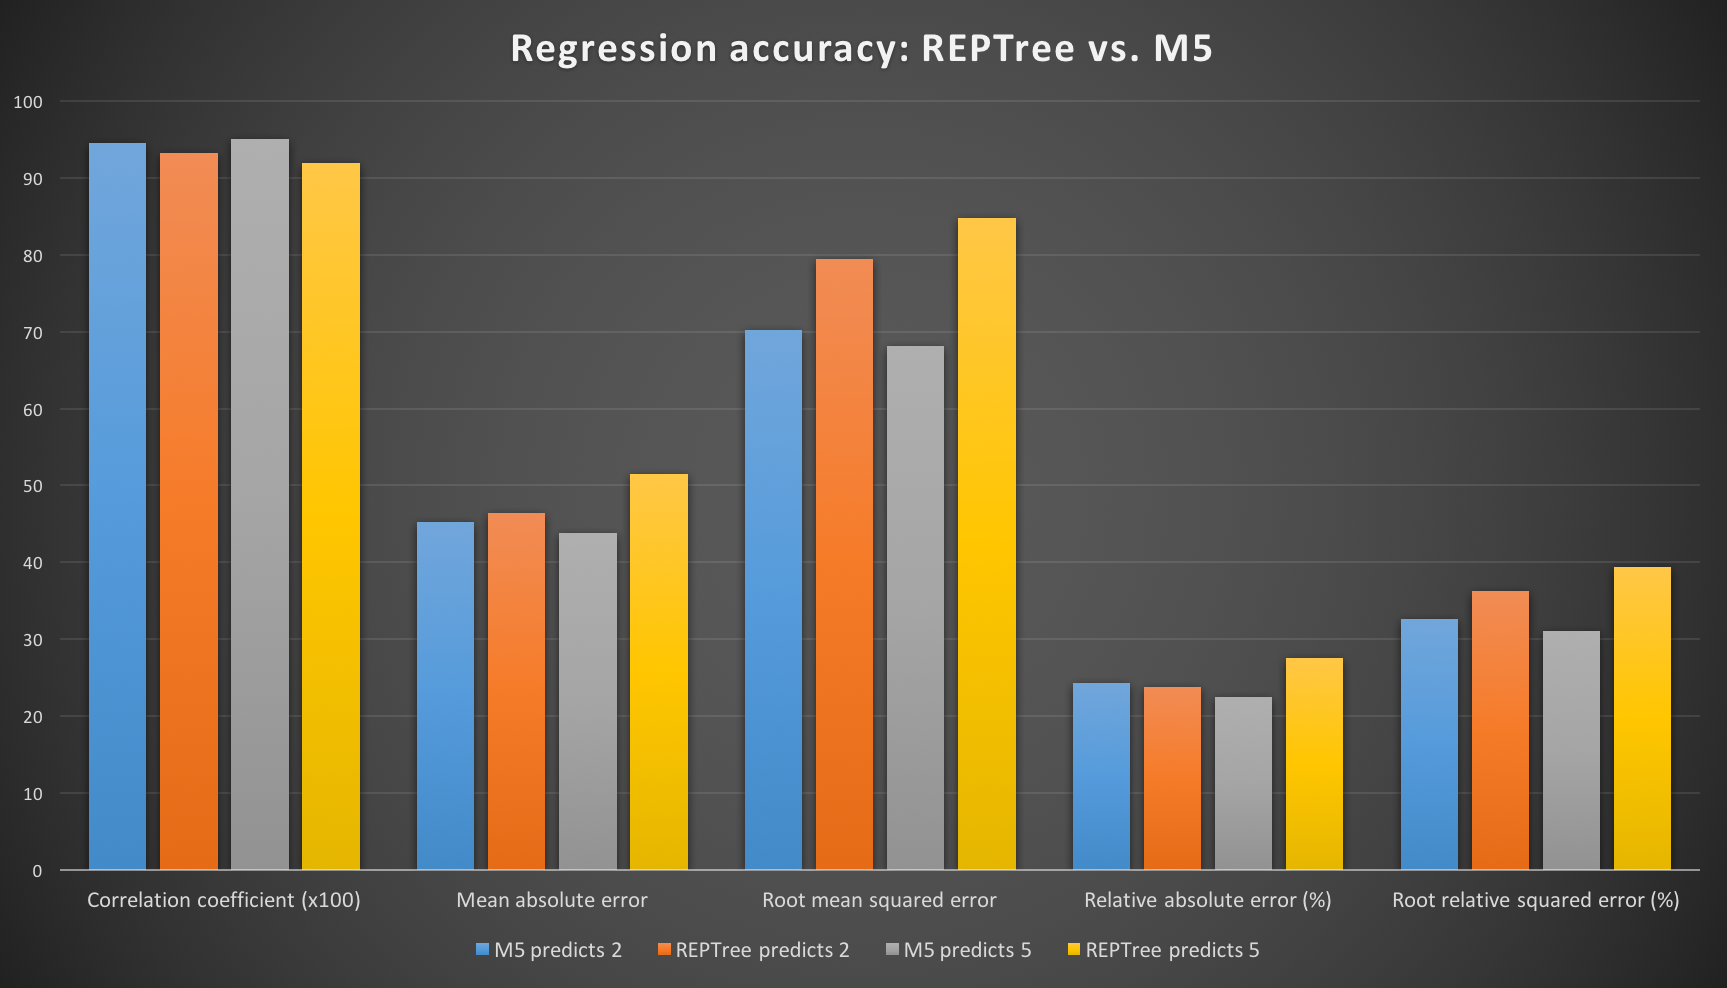
\includegraphics[width=\textwidth]{REPTree_vs_M5}

\vspace{0.3cm}

Observamos que \emph{M5} reduce de forma visible el error en la predicción a la vez que eleva el coeficiente de correlación, y es por ello que será éste el algoritmo que implementaremos a continuación.

\subsection{Implementación}

Dado que en el anterior apartado hemos usado el wrapper de \emph{Weka} para implementar nuestro agente, en este hemos decidido implementar las reglas \emph{a mano} para poder valorar ambas alternativas. \emph{M5}, algoritmo empleado en esta implementación, genera reglas que devuelven un valor para la clase dando pesos a cada uno de los demás atributos a modo de coeficientes para posteriormente sumar cada valor multiplicado por dicho coeficiente.

Este tipo de reglas no nos supone mucha dificultad a la hora de implementarlas en nuestro método de recolección de datos. El procedimiento a seguir con tal fin es sustituir las variables que aparecen en la regla por aquellas que contienen los datos requeridos, e ir poniendo una regla tras otra a modo de \texttt{if-else} en el código.

\newpage
\section{Preguntas propuestas}

\begin{center}
    \emph{¿Qué diferencias hay a la hora de aprender esos modelos con instancias provenientes de un agente controlado por un humano y uno automático?}
\end{center}

Los datos de las instancias provenientes de nuestro agente automático del \emph{Tutorial 1} contienen numerosos movimientos que podríamos calificar como ``malos'', o que no nos acercan al objetivo. Estas instancias causan ruido a la hora de generar un modelo de clasificación, provocando clasificaciones que no acercan a \emph{PacMan} a los fantasmas.

Por el contrario, los datos recolectados con nosotros jugando contienen muchos menos de estos datos de movimientos que dan \emph{palos ciegos} dado que el agente en este caso humano está mucho más informado al poder ver a los fantasmas, generando un modelo de clasificación mucho más preciso.

\begin{center}
     \emph{¿Crees que los resultados del modelo de regresión a 5 turnos vista guardan relación con los de 2 turnos? ¿Por qué?}
\end{center}

Los resultados de los modelos de regresión a 2 y 5 turnos vista están relacionados hasta el punto de ser posible generalizar dichos modelos a $N$ turnos vista. Esto es así porque los modelos basan su predicción en dos hechos: el primero que, por cada turno que pasa, la puntuación desciende en una unidad siempre; el segundo, la probabilidad de \emph{cazar} fantasmas en los turnos venideros, y ambos datos son calculables tanto para 2, como para 5, como para cualquier otro número positivo.

\begin{center}
     \emph{Si quisieras transformar la tarea de regresión en clasificación ¿Qué tendrías que hacer? ¿Cuál crees que podría ser la aplicación práctica de predecir la puntuación?}
\end{center}

Para esto, se \textbf{\emph{discretizan}} los valores de salida mediante el filtro correspondiente en \emph{Weka}. Dado que la puntuación es el dato a maximizar, predecir la puntuación futura puede ser útil si los datos que se han usado para obtener el modelo de predicción vienen de partidas en las que se haya jugado bien. De esta forma se podría determinar si una serie de movimientos ha sido correcta o no dependiendo de la desviación de la puntuación respecto a la predicción.

\begin{center}
     \emph{¿Qué ventajas puede aportar predecir la puntuación respecto a la clasificación de la acción? Justifica tu respuesta.}
\end{center}

La ventaja real de predecir la puntuación reside en su uso para predecir la clasificación de la acción. Es una herramienta más para ayudar al clasificador, sin utilidad por sí misma.

\begin{center}
    \emph{¿Crees que se podría conseguir alguna mejora en la clasificación incorporando un atributo que indicase si la puntuación en el instante actual ha descendido o ha bajado?}
\end{center}

La inclusión de un atributo que indicase la variación de la puntuación respecto al turno anterior es una manera más de acercarse a nuestro planteamiento de clasificar los movimientos tomados como \emph{buenos} o \emph{malos}. Esto puede resultar muy útil a la hora de filtrar los datos, si bien no nos sirve como única métrica dado que un movimiento no sólo es bueno si incrementa la puntuación sino que también lo es cuando acerca a \emph{PacMan} a los fantasmas.
\vspace{-0.3cm}

\newpage
\section{Conclusiones}

Si bien el aprendizaje automático es una técnica bien aplicable al problema de jugar al \emph{PacMan}, los datos con los que cuenta el agente parecen escasos para el desarrollo satisfactorio de esta tarea, dados los resultados de juego. El modelo actual puede ser útil para una de las partes de la que debería constar un agente, como es la evaluación de los movimientos, debido a la interacción con la puntuación futura a $N$ turnos vista. Sin embargo, no nos parece suficiente esto para generar un agente realmente bueno para jugar al \emph{PacMan}.

Un dominio que nos resulta interesante para explorar a la hora de mejorar nuestro agente es la planificación de objetivos. Así, para cada mapa, podríamos decidir qué ruta seguir hasta nuestro objetivo. Si bien el agente automático no tiene datos sobre la posición exacta de los fantasmas, sí tiene un vector de distancias que podría ser utilizado para \emph{predecir} dónde podrían estar cada uno de ellos, en conjunción con la información que nos proporcionen los movimientos que hagamos. Una vez predicha la posible esa posición, se podrían buscar rutas directas hasta el objetivo, evitando así los bloqueos de \emph{PacMan} cuando se encuentra en una cárcel (muros en forma de \emph{U} que encierran a \emph{PacMan} cuando quiere avanzar hacia un objetivo que se encuentra al otro lado de la base).

Estos acercamientos, al igual que otros muchos, podrían ayudarnos a conseguir un agente que realmente juegue bien e incluso mejor que un ser humano pues, de momento, este no es el caso.

\vspace{0.2cm}

\centerline{\textbf{Problemas encontrados}}

\vspace{0.5cm}

La integración de \emph{Weka} en \texttt{Python} nos pareció una idea muy interesante para encarar un entorno lo más real posible; sin embargo, como no era un objetivo \emph{per se} de la práctica, supuso un proceso de investigación previo y la adaptación a un \emph{framework} nuevo.

Si bien éste es un objetivo de la práctica original de la \emph{Universidad de California}, hemos echado en falta el algoritmo de predicción de la posición de los fantasmas, como justificamos anteriormente. Por nuestra cuenta encontramos dicha implementación y comprobamos que verdaderamente resultaba en un aumento considerable del éxito en la predicción.

Cabe mencionar también que la abundante carga de trabajo debida a la suma de otras asignaturas en la que nos hallamos matriculados nos ha restringido el tiempo que hemos podido dedicar a esta práctica, dejándonos bastante menos del que nos hubiera gustado.

\vspace{0.5cm}

\centerline{\textbf{Comentarios personales}}

\vspace{0.5cm}

En oposición a los anteriores \emph{Tutoriales}, que guiaban mucho más al alumno, llegaron algunos momentos en los que nos encontramos \emph{perdidos} o \emph{estancados}, sin saber muy bien qué paso era el próximo a tomar. Sin embargo, creemos que con trabajo y una actitud proactiva completamos satisfactoriamente todas las partes de las que constaba esta práctica.

\end{document}
